
\chapter{Projekt i implementacja strony serwerowej opartej na architekturze REST w technologi Django oraz bazy danych MySQL}
\section{Narzędzia i techonologie}
\subsection{Django}
Django~\cite{Django} jest darmową, wysokopoziomową platformą programistyczną przeznaczoną do tworzenia aplikacji internetowych. Dostarcza wiele narzędzi ułatwiających szybką oraz prostą implementację. Oparta jest na wzorcu architektonicznym model-template-view~(zob.~rysunek~\ref{rys:django}). Napisana jest w języku Python. Jednymi z najważniejszych cech Django są:
\begin{itemize}
	\item łatwy i bezpieczny dostęp do bazy danych,
	\item duża skalowalność oraz wydajność,
	\item wbudowane zabezpieczenia przed popularnymi, atakami
	\item rozbudowana dokumentacja.
\end{itemize}
\begin{figure}[H]
	\centering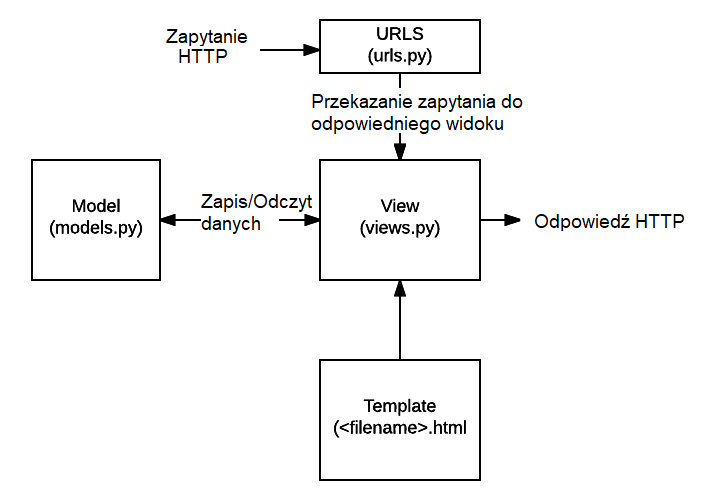
\includegraphics[width=\textwidth]{figures/DjangoSchemat}
	\caption{Schemat przepływu danych w Django~\cite{DjangoSchemat}}\label{rys:django}
\end{figure}
\subsection{MySQL}
MySQL~\cite{SQL} jest systemem służącym do zarządzania relacyjnymi bazami danych. Model relacyjny zapewnia łatwość w projektowaniu oraz implementacji. Udostępniony jest na licencji wolnego oprogramowania i dostępny jest dla wszystkich popularnych systemów operacyjnych. Bazy danych oparte na tym systemie są wstanie obsługiwać olbrzymie liczby zapytań w bardzo krótkim czasie.
\subsection{MySQL Workbench}
MySQL Workbench~\cite{Workbench} to narzędzie do projektowania, tworzenia oraz zarządzania bazami danych MySQL. Posiada bardzo przejrzysty i intuicyjny interfejs, przez co cieszy się dużą popularnością. Wiele podstawowych czynności takich jak np. tworzenie i edycja tabel, można wykonać bez znajomości zapytań SQL, gdyż są one generowane automatycznie.

\section{Implementacja serwera REST API}
\subsection{REST}
REST ~\cite{REST} jest stylem architektonicznym wprowadzającym pewien standard komunikacyjny dla internetowych systemów informatycznych~(zob.~rysunek~\ref{rys:rest}). Jego najważniejszymi zaletami są szybkość oraz uniwersalność. Interfejsy programistyczne spełniające założenia REST mogą komunikować się z dowolnym urządzeniem sieciowym, pod warunkiem wysyłania przez nie zapytań w odpowiednim formacie. Jednymi z głównych zasad tego stylu są:
\begin{itemize}
	\item zastosowanie modelu klient-serwer,
	\item bezstanowość,
	\item wykorzystywanie pamięci cache przeglądarki w celu zapamiętywania odpowiedzi,
	\item interfejs programistyczny jednolity dla każdej aplikacji klienckiej.
\end{itemize}
\begin{figure}[H]
	\centering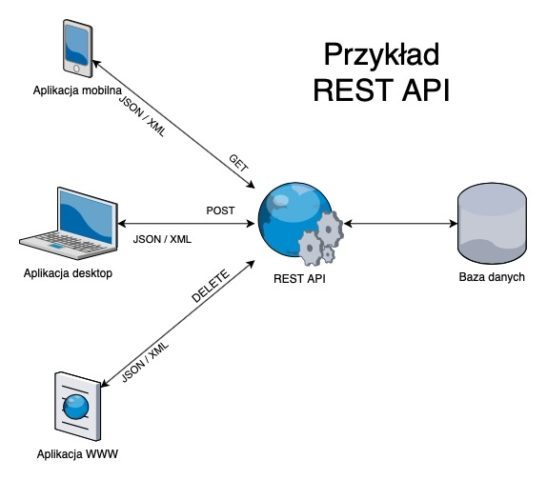
\includegraphics[width=\textwidth]{figures/rest}
	\caption{Przykładowy schemat działania REST API~\cite{SchematRest}}\label{rys:rest}
\end{figure}

Zapytania zazwyczaj wysyłane są przy pomocy protokołu HTTP. Zarówno do zapytań, jak i do odpowiedzi, najczęściej wykorzystywane są metody GET oraz POST. Informacje przesyłane między klientem a serwerem muszą być precyzyjne, zwykle występują one w formacie JSON. 

\subsection{Modele}
Jednym z najważniejszych mechanizmów zaimplementowanych w Django są modele. Są one swego rodzaju mapowaniem klas języka Python na tabele bazy danych. Takie rozwiązanie zapewnia bardzo szybki i wygodny dostęp do przechowywanych informacji. Klasy te zdefiniowane są w pliku ,,models.py''. Wykorzystując wbudowane funkcje wykorzystywanej platformy programistycznej, można zarówno wygenerować tabele bazy danych na podstawie modeli, jak i wygenerować modele na podstawie gotowych tabel.

W projekcie znajduje się następujących siedem modeli: 
\begin{itemize}
	\item Classrooms,
	\item Lessons,
	\item Planners,
	\item Polls,
	\item Subjects,
	\item Teachers,
	\item Timetables.
\end{itemize}
Każdy odpowiada jednej tabeli z bazy danych, pola w każdej z klas są analogiczne do kolumn w odpowiednich tabelach. Zawierają informacje takie jak np. typ danych, maksymalna długość oraz klucz główny.
Implementacja przykładowej klasy:
\begin{figure}[H]
	\centering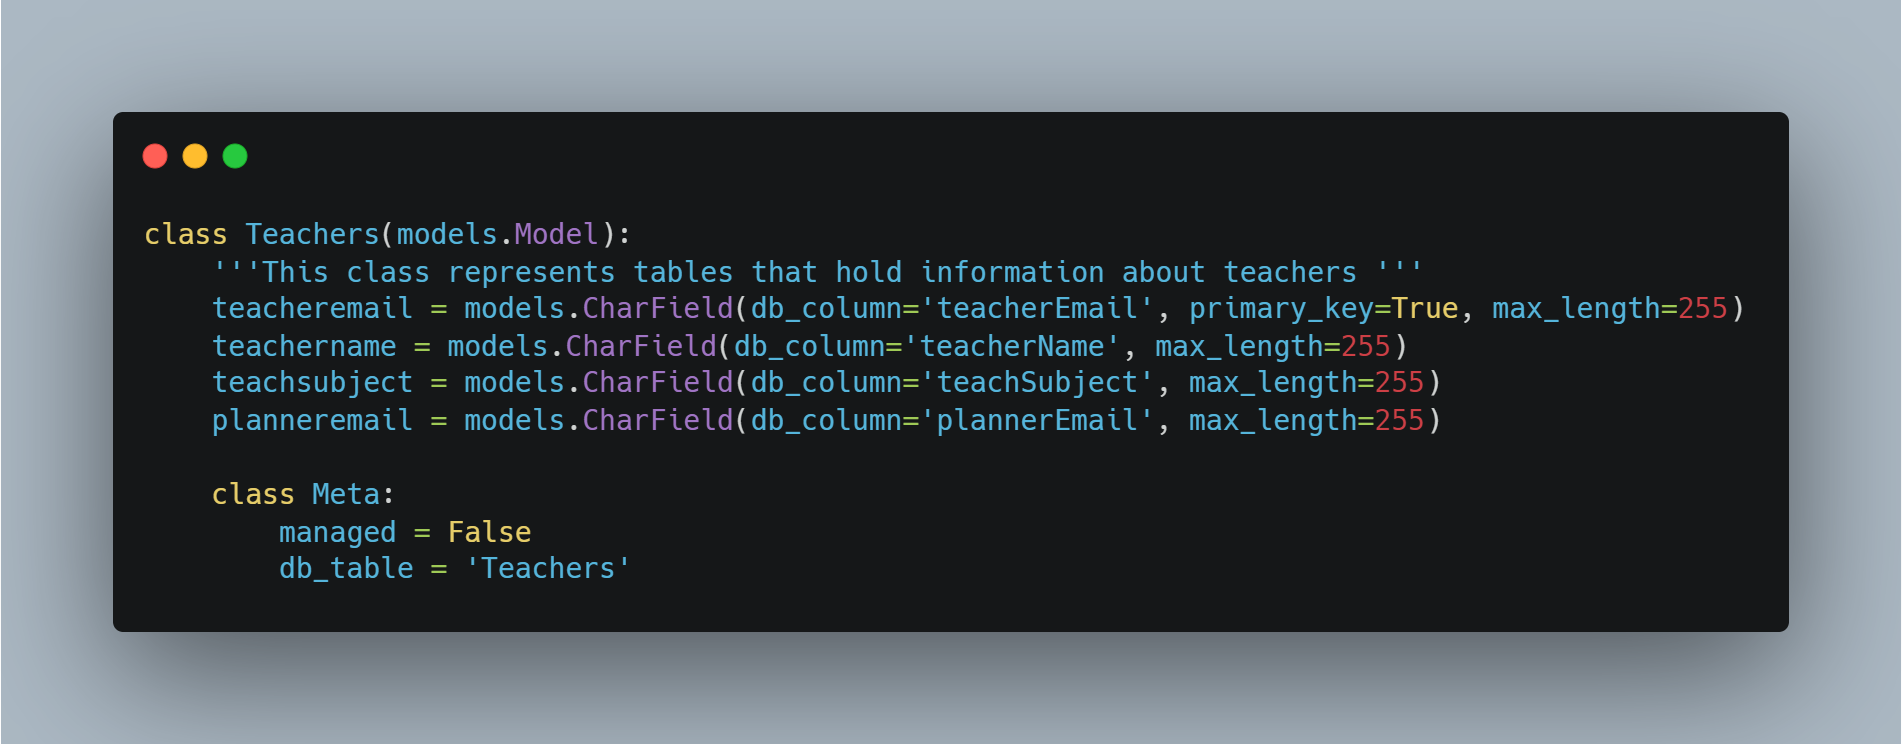
\includegraphics[width=\textwidth]{figures/TeachersModel}
	\caption{Implementacja klasy Teachers}\label{rys:TeachersModel}
\end{figure}

\subsection{Adresy internetowe}
Kolejnym elementem implementacji są adresy internetowe. W pliku ,,urls.py'' określone zostały wykorzystywane w projekcie adresy URL, oraz funkcje, które mają zostać wywołane w przypadku otrzymania od klienta zapytania na dany adres. Implementacja adresów przedstawiona została na rysunku ~\ref{rys:URLs}
\begin{figure}[H]
 	\centering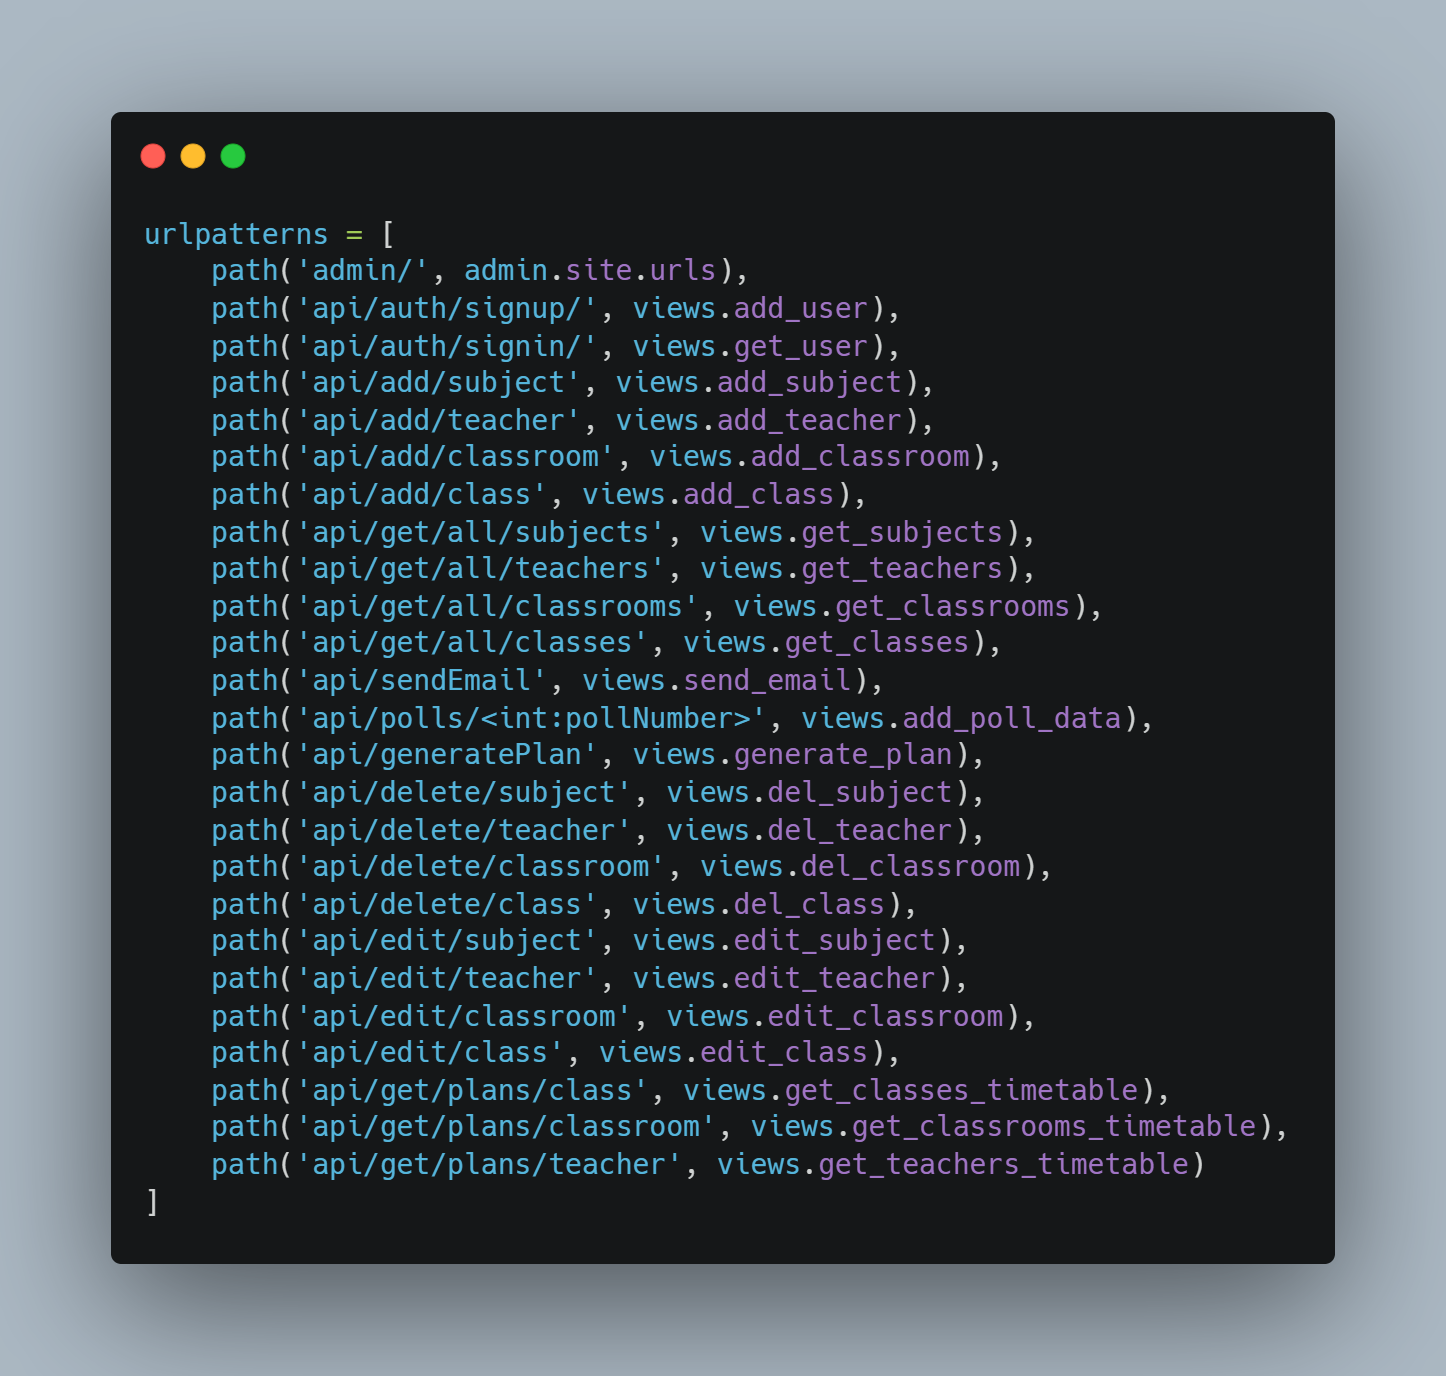
\includegraphics[width=\textwidth]{figures/Urls}
 	\caption{Implementacja adresów URL}\label{rys:URLs}
\end{figure}
W przypadku, jeśli zapytanie przyjdzie na niezadeklarowany adres, zwrócony zostanie komunikat HTTP z kodem 404(Page Not Found).

\subsection{Widoki}
Widoki to nic innego, jak funkcję języka Python wykonywane w momencie odbioru zapytania przez serwer. Kiedy klient wyśle zapytanie na dany adres, Django sprawdza, czy jest on zadeklarowany we wspomnianym wcześniej pliku ,,urls.py'', jeśli tak, to wywoływana jest odpowiednia funkcja z pliku ,,views.py'' wraz z jej parametrem którym jest samo zapytanie. Dzięki takiej parametryzacji, widok ma łatwy dostęp do otrzymanych informacji, sprawdza on czy są one prawidłowe, oraz wykonuje na nich odpowiednie działania. W tym projekcie, w większości przypadków wykonywane są operacje zapisu i odczytu z bazy danych. Do komunikacji wykorzystywane są metody GET oraz POST z protokołu HTTP.
Implementacje przykładowych widoków obsługujacych zapytania dla danych metod HTTP przedstawione zostały na rysunkach ~\ref{rys:BackendGet} oraz ~\ref{rys:BackendPost}
\begin{figure}[H]
	\centering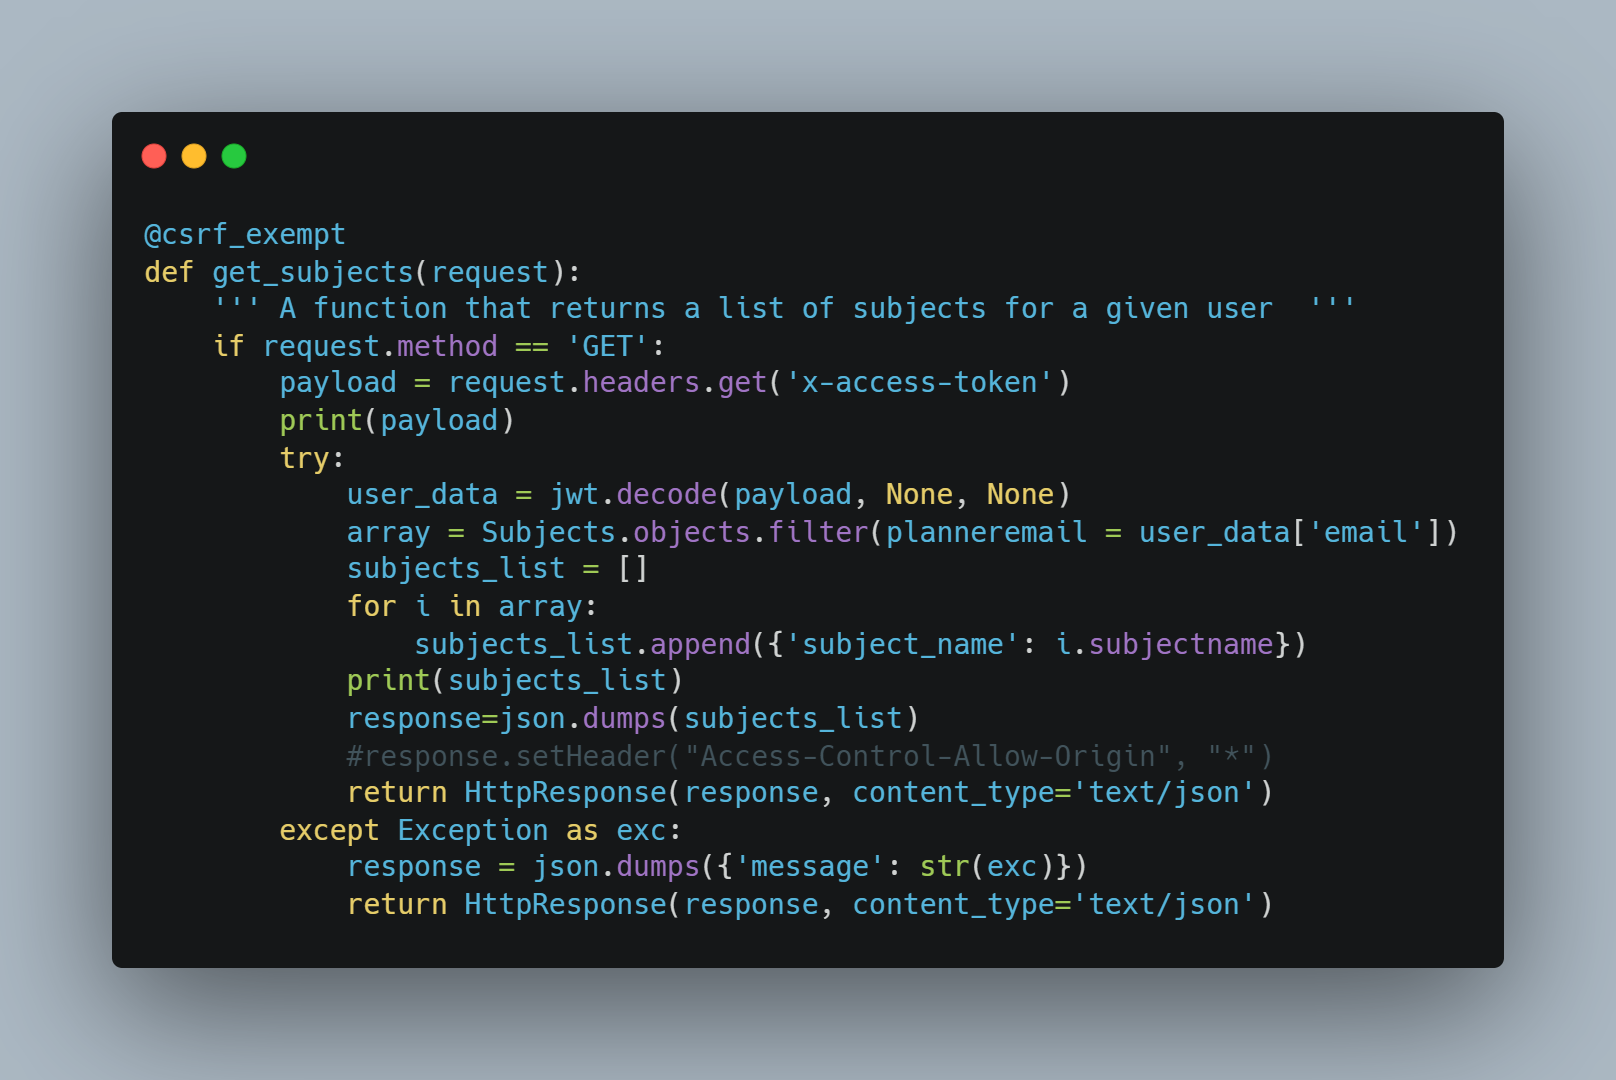
\includegraphics[width=\textwidth]{figures/BackendGet}
	\caption{Widok obsługujący zapytanie typu GET}\label{rys:BackendGet}
\end{figure}
\begin{figure}[H]
	\centering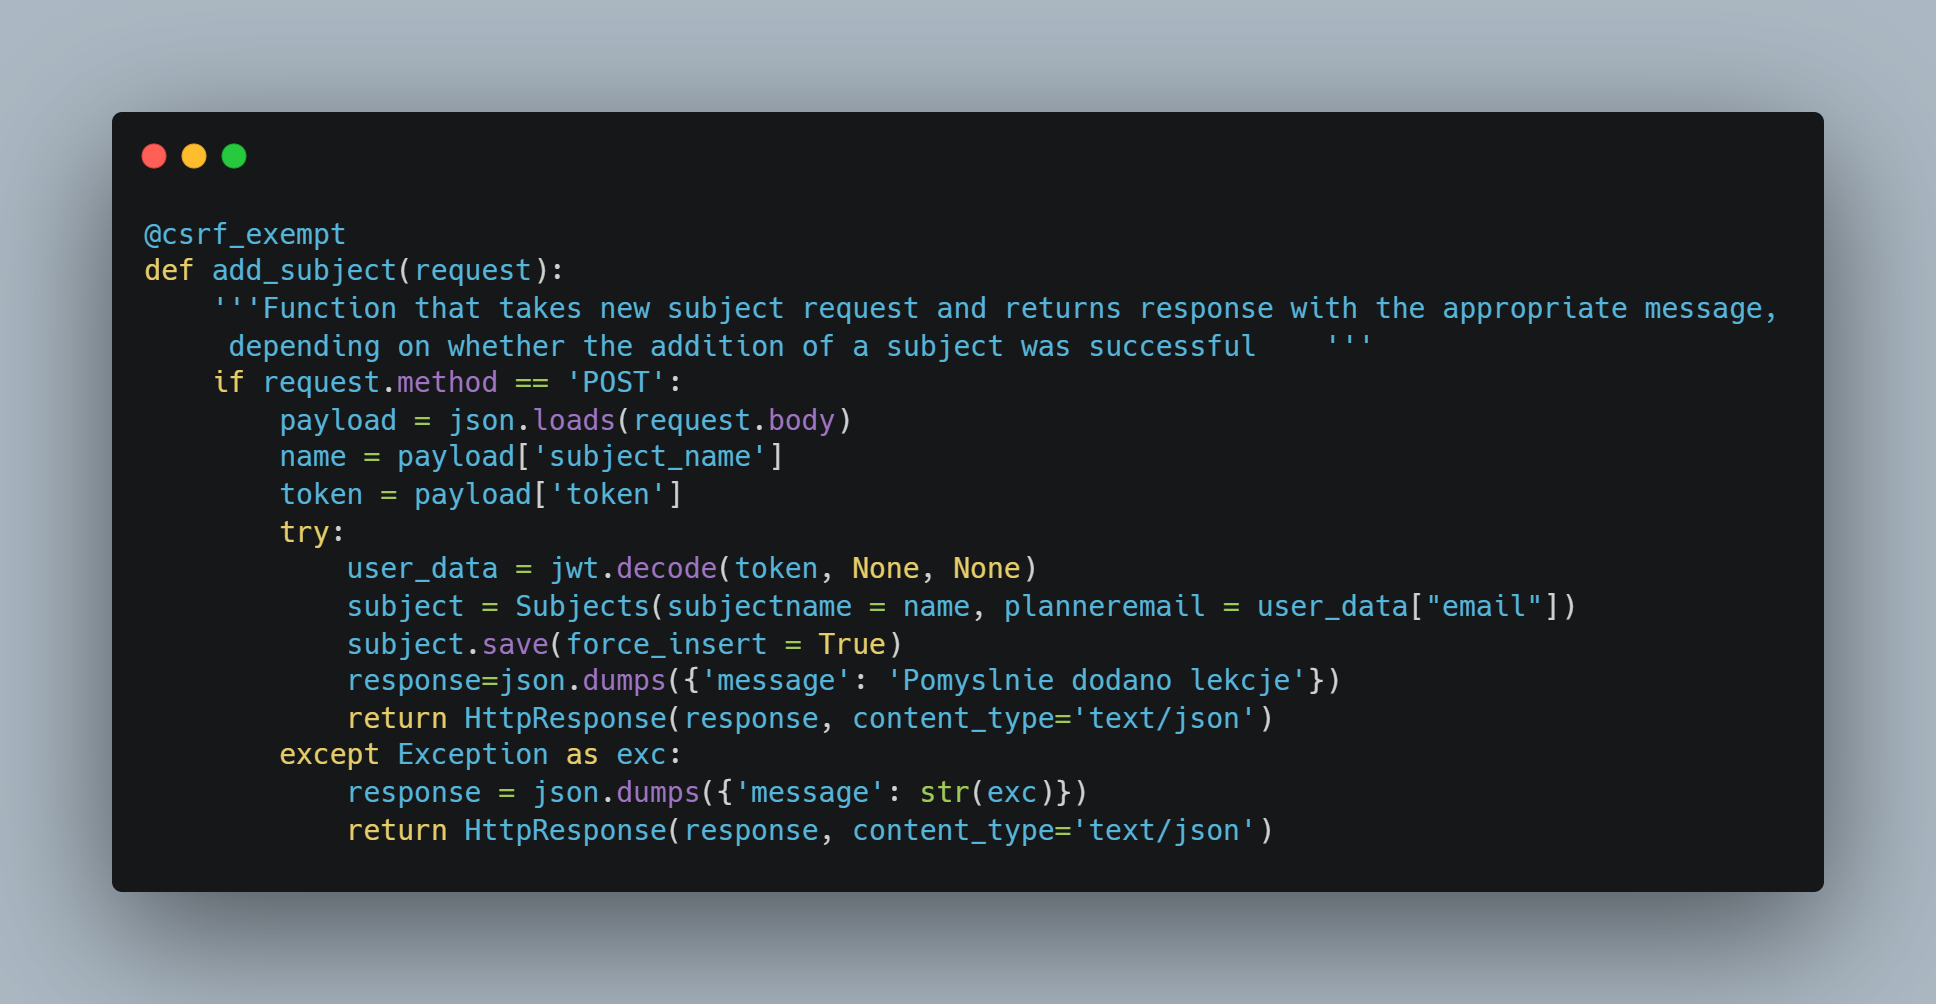
\includegraphics[width=\textwidth]{figures/BackendPost}
	\caption{Widok obsługujący zapytanie typu POST}\label{rys:BackendPost}
\end{figure}

\section{Główne funkcjonalności}
\subsection{Rejestracja i logowanie}
Rejestracja oraz logowanie zrealizowane są za pomocą dwóch adresów, co za tym idzie również dwóch widoków, obsługujących zapytania z metodą POST. Do zarejestrowania nowego użytkownika wymagane jest podanie danych takich informacji jak adres e-mail, login oraz hasło. Funkcja obsługująca rejestrację zapisuje te dane do odpowiedniej tabeli, pod warunkiem że dany użytkownik nie istnieje już w bazie danych, a następnie zwraca odpowiedni komunikat. W przypadku logowania wymagane jest podanie adresu e-mail oraz hasła podanych przy rejestracji. Jeśli podane dane są poprawne, generowany oraz zwracany klientowi jest token (JWT). Zakodowane w nim są wszystkie dane podane przy rejestracji, co pozwala na identyfikację użytkownika przy dalszej komunikacji. Generacja JWT na rysunku ~\ref{rys:jwt}. 
\begin{figure}[H]
	\centering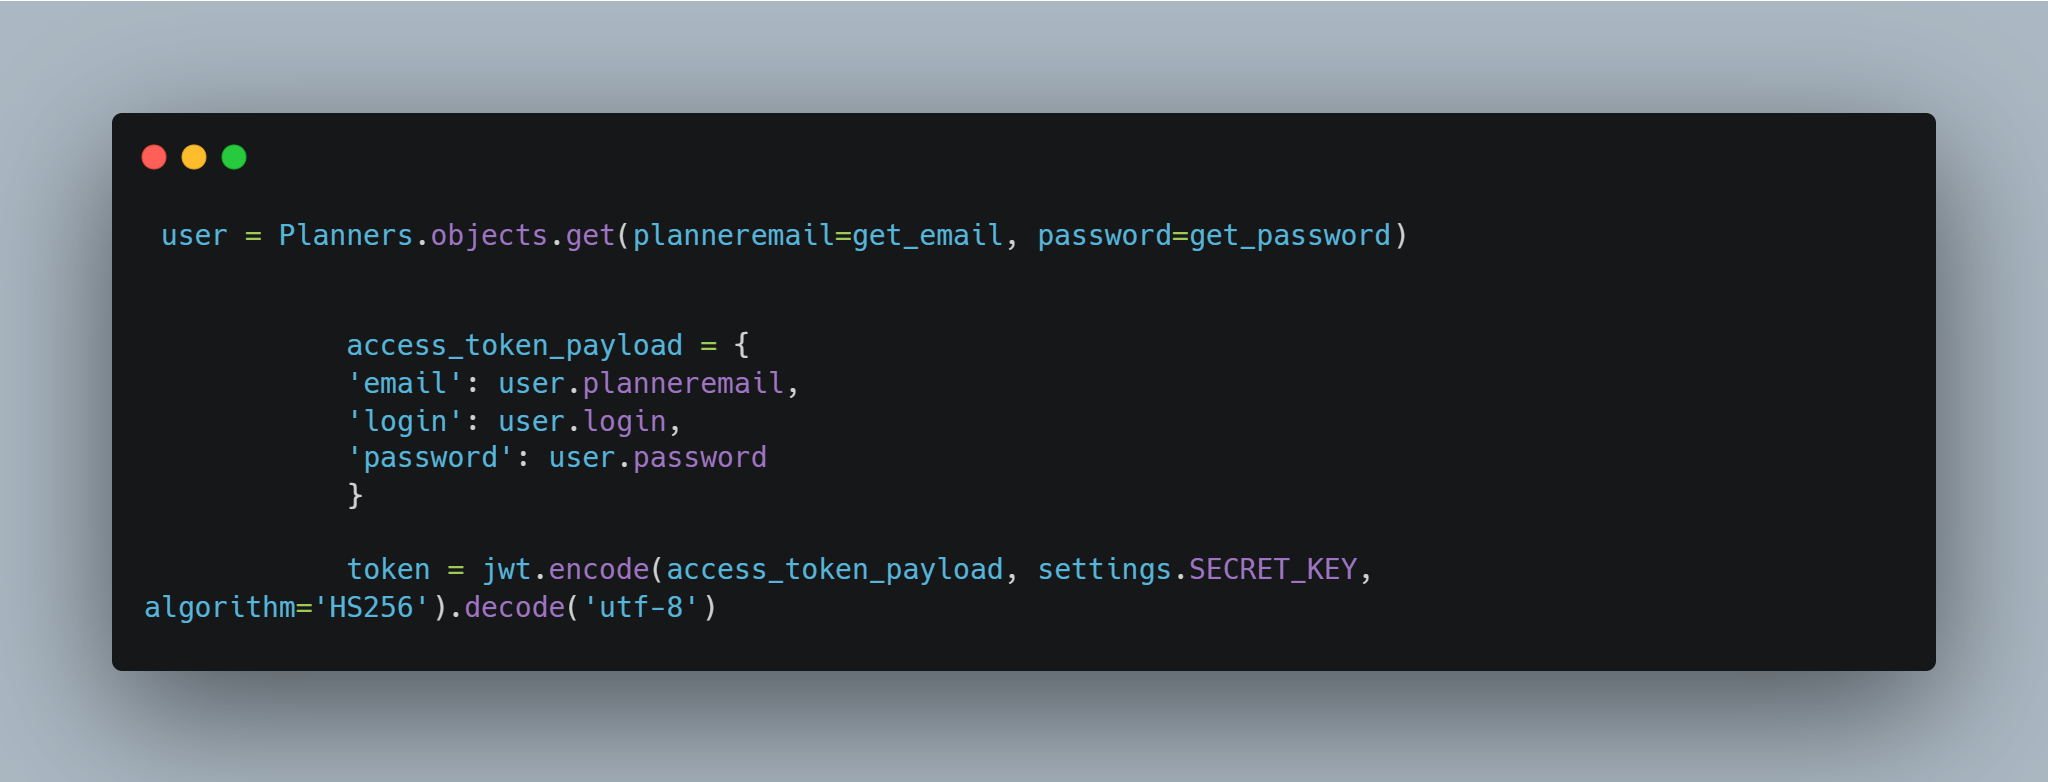
\includegraphics[width=\textwidth]{figures/jwt}
	\caption{Fragment kodu generujący JWT}\label{rys:jwt}
\end{figure}
\subsection{Uzupełnianie danych potrzebnych do generacji planu}
Dane które są wymagane do generacji planu lekcji, można podzielić na 4 grupy:
\begin{itemize}
	\item nauczyciele,
	\item klasy,
	\item sale lekcyjne,
	\item przedmioty.
\end{itemize}
W projekcie zaimplementowane są widoki, pozwalające dodawać, edytować, usuwać oraz zwracać informacje o każdej z tych grup. W większości przypadków są to proste operacje zapisu i odczytu z bazy danych, jednak w przypadku dodawania informacji o nauczycielach istnieje dodatkowa funkcjonalność, pozwalająca na wysłanie do nich wiadomości e-mail z adresem do indywidualnej ankiety, w której można określić preferowane godziny pracy. Przy pomyślnej realizacji zapytania o wysłanie wiadomości e-mail, w bazie danych tworzone są wiersze, do których zapisane będą dane z ankiet. Są one identyfikowane po unikatowym numerze, przekazywanym jako parametr w adresie URL. Dzięki takiemu rozwiązaniu, generowany jest indywidualny link do ankiety dla każdego nauczyciela.
\subsection{Generacja oraz zwracanie planów}
Generacja oraz zwracanie planów zrealizowane są za pomocą czterech widoków. Funkcja generacji planu ma za zadanie odczytać wszystkie potrzebne informacje i w odpowiednim formacie przekazać je do generatora. Ze względu na to, że klient nie powinien oczekiwać na odpowiedź oraz że czas generacji planu może być stosunkowo długi, widok ten w przypadku pomyślnego przygotowania danych wejściowych, zwraca informację o rozpoczęciu generacji planu, nie czekając na zakończenie procesu. Dzięki temu, proces generacji nie zaburza połączenia klient-serwer. Kiedy generator skończy pracę, plany lekcji zapisywane są w bazie danych w trzech wersjach, z perspektywy: klas, nauczycieli oraz sal lekcyjnych.
Każdy z tych planów, jest zwracany za pomocą pozostałych trzech widoków.

\section{Baza danych MySQL}